% Vorlesung vom 17.12.2015
\renewcommand{\ldate}{2015-12-17}
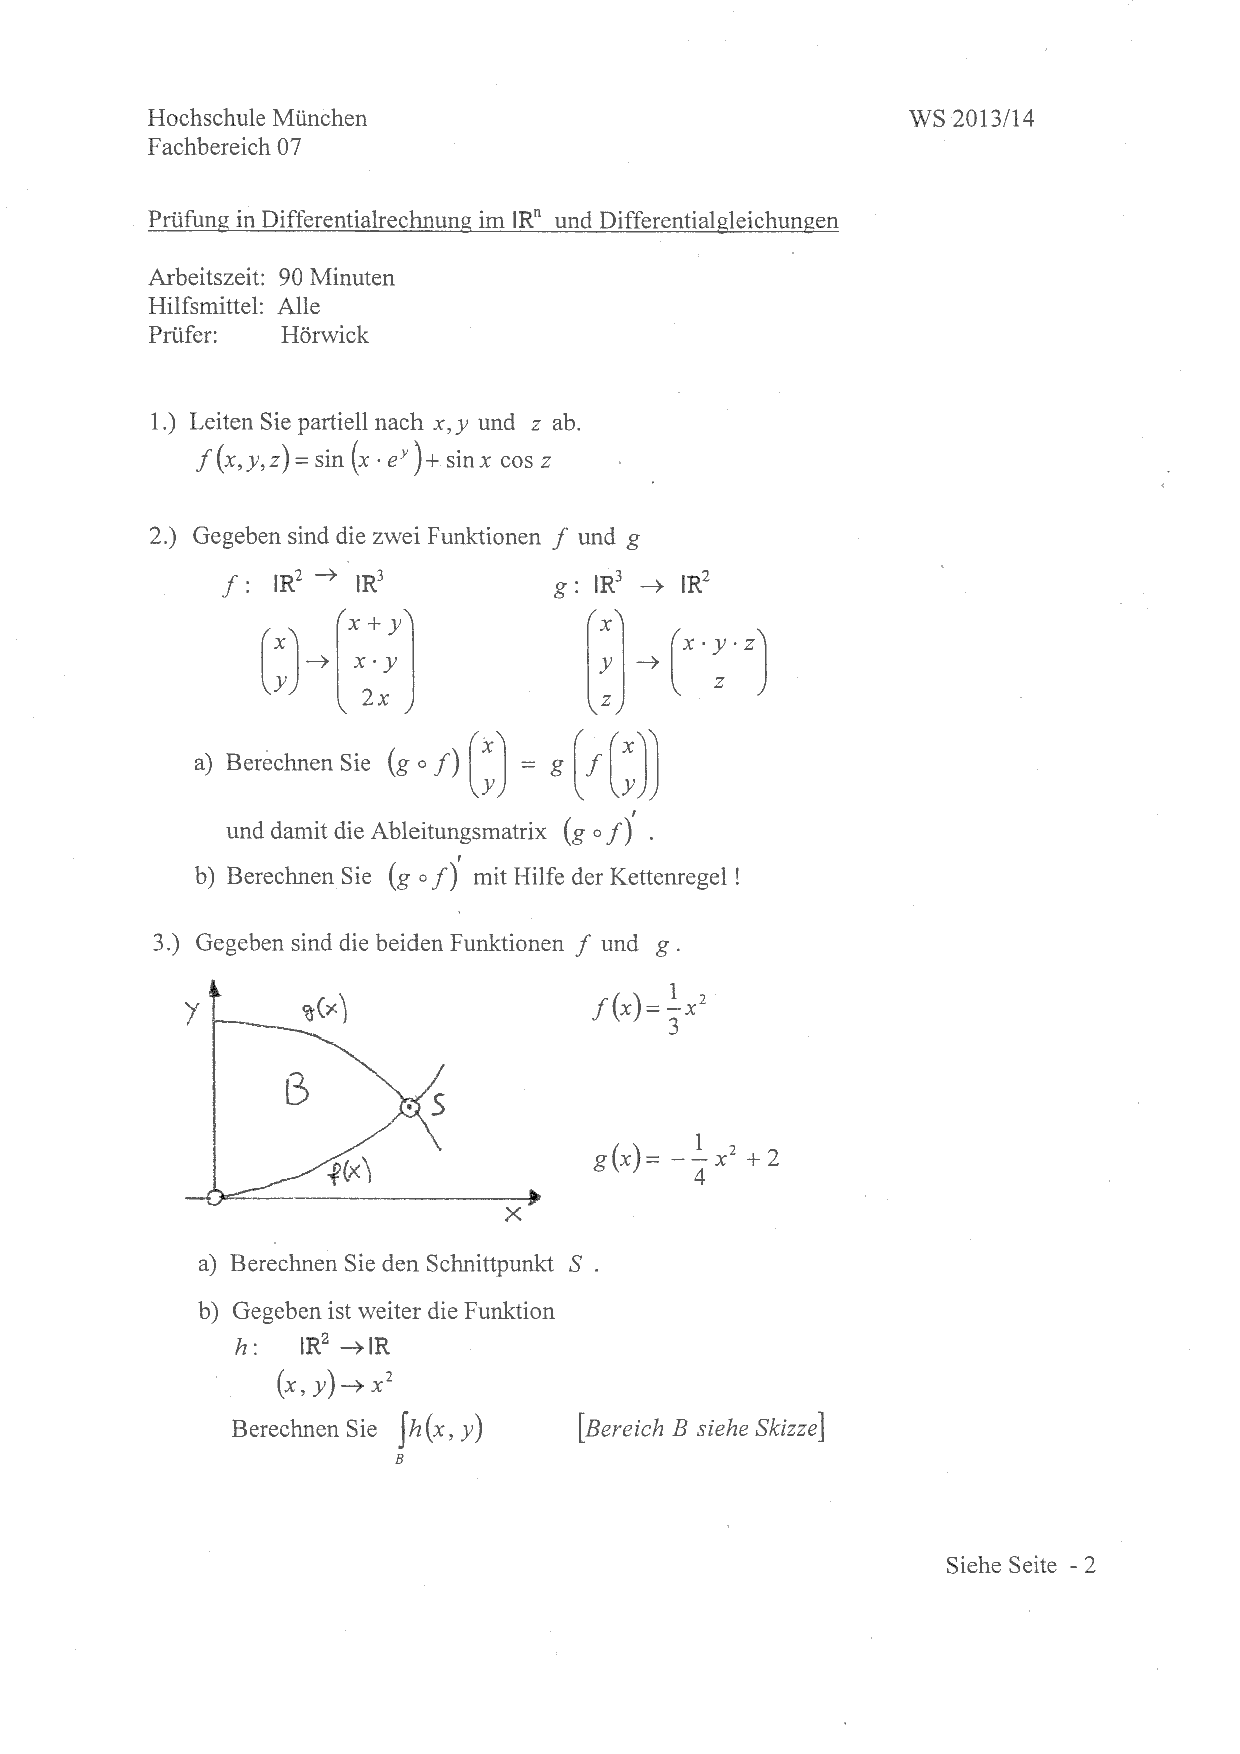
\includepdf[pages=-]{pruefungsangabe_ws1314}

\section{Lösung für die Prüfung WS 2013/14}

\subsection{zu 1)}
$f(x,y,z)$
$=\sin(x\cdot e^y) + \sin x \cos z$

$\frac{\df}{\dx} = \cos (x\cdot e^y) e^y + \cos x \cos z$

$\frac{\df}{\dy} = \cos (x\cdot e^y) x e^y $

$\frac{\df}{\dz} = -\sin x \sin z$

\subsection{zu 2a)}
$ (g\circ f) \vektor{x\\y} $
$= g\vektor{x+y\\x\cdot y\\2x}$
$=\vektor{(x+y) x y 2 x \\ 2x}$
$=\vektor{2x^3y + 2x^2y^2\\2x}$

\textbf{Ableitungsmatrix:}
$ (g\circ f)' \vektor{x\\y} $
$=\vektor{6yx^2 + 4xy^2, 2x^3 + 4x^2y\\2, 0}$

\subsection{zu 2b)}
$f'\vektor{x\\y}$
$=\vektor{1,1\\y,x\\2,0}$

$g'\vektor{x\\y\\z}$
$=\vektor{yz, xz, xy\\0,0,1}$

$
(g\circ f)' \vektor{x\\y} 
=g' \rbr{f \vektor{x\\y}}  \cdot f'\vektor{x\\y}
=g'\vektor{x+y\\x\cdot y\\2x}  \cdot \vektor{1,1\\y,x\\2,0} 
=\vektor{2x^2y, 2x^2+2xy,x^2y+y^2x\\0,0,1} \cdot \vektor{1,1\\y,x\\2,0} 
=...=\vektor{6yx^2 + 4xy^2, 2x^3+4x^2y\\2,0}
$\profnote{Matrizenmultiplikation: Zeile mal Spalte!}

\subsection{zu 3a)}
$f(x) = g(x)$

$\frac{1}{3} x^2 = -\frac{1}{4} x^2 + 2$

$x=1.85 \Rightarrow y = f(1.85) = 1.14 \Rightarrow S(1.85, 1.14)$

\subsection{zu 3b)}
$
\int_{B} h(x,y) 
=\int_{0}^{1.85} \rbr{\int_{f(x)}^{g(x)} h(x,y) dy} dx
=\int_{0}^{1.85} \rbr{ \int_{\frac{1}{3} x^2}^{-\frac{1}{4} x^2 + 2} x^2 dy} dx
=\int_{0}^{1.85} \sbr{yx^2}_{y=\frac{1}{3} x^2}^{y=-\frac{1}{4} x^2 + 2} dx
=\int_{0}^{1.85} \rbr{\rbr{-\frac{1}{4} x^2 + 2} x^2 - \frac{1}{3} x^2 x^2} dx
=\int_{0}^{1.85} -\frac{1}{4} x^4 + 2x^2 - \frac{1}{3} x^4 dx
=\int_{0}^{1.85} -\frac{7}{12} x^4 + 2x^2 dx
=\sbr{-\frac{7}{12} \cdot \frac{1}{5} x^5 + 2\cdot \frac{1}{3} x^3}_0^{1.85} 
=-\frac{7}{60} \cdot 1.85^5 + \frac{2}{3} \cdot 1.85^3
=1.69
$

% Vorlesung vom 18.12.2015
\subsection{zu 4a)}
\underline{$\varphi(0) = 1$}

$\varphi'(x) = x^2+(x-1)\cdot \varphi(x)$

\underline{$\varphi'(0) = -1$}

$\varphi''(x) = 2x + 1\cdot \varphi(x) + (x-1)\cdot \varphi'(x)$ \profnote{Produktregel!}

$\varphi''(0) = 1 + (-1) \cdot (-1) = 2$

$\varphi'''(x) = 2+\varphi'(x) + \varphi'(x) + (x-1)\cdot \varphi''(x)$

$\varphi'''(0) = 2-1-1+(-1)\cdot 2 = -2	 $

\subsection{zu 4b)}
$\varphi(h) \approx \varphi(0) + \varphi'(0) \cdot h + \frac{\varphi''(0)}{2!} \cdot h^2 + \frac{\varphi'''(0)}{3!} \cdot h^3$

$\varphi(h) \approx 1 + (-1)\cdot h + \frac{2}{2} \cdot h^2 + \frac{-2}{6} \cdot h^3$

$\varphi(0.1) \approx 1 - 0.1 + 0.1^2 - \frac{1}{3} \cdot 0.1^3 $

$\varphi(0.1) \approx 0.9097$

\subsection{EXTRA zu 4)}
Löse $y' = \underbrace{(x-1)}_{a} \cdot y + \underbrace{x^2}_{b}, \varphi(0) = 1$. Ist vom Typ lineare DGL. 

\textbf{Lösungsweg:} \profnote{Aus dem Skript}
\begin{enumerate}
\item $\varphi(x) = exp\rbr{\int_{x_0}^{x} a(t) dt}$
\item $\psi(x) = \varphi(x) \cdot \sbr{c + \int_{x_0}^{x} \frac{b(t)}{\varphi(t)} dt}$
\end{enumerate}

\textbf{Lösung}

$
\varphi(x) = exp\rbr{\int_{0}^{x} t-1 dt}
=exp\rbr{\sbr{\frac{1}{2} t^2 - t }_0^x}
=exp\rbr{\frac{1}{2} x^2 - x}
$

$ \psi(x) = exp(\frac{1}{2} x^2 - x) \cdot \sbr{1 + \underbrace{\int_{0}^{x} \frac{t^2}{exp(\rbr{\frac{1}{2} t^2 - t})}}_{f(t)} dt} $. 
$\varphi(x)$ ist die Lösung. Näherung für das Integral von 0 bis 0.1: 

$
f(0)=0, f(0.1) = \frac{0.1^2}{exp\rbr{\frac{1}{2} \cdot 0.1^2 - 0.1}} = 0.011
\Rightarrow \int_{0}^{0.1} ... dt = 0.1 \cdot \frac{1}{2} (0+0.011) = 0.00055
\Rightarrow \psi(0.1) = exp\rbr{\frac{1}{2} \cdot 0.1^2 - 0.1} \sbr{1+0.00055} = 0.90987
$

\subsection{zu 5)}
Substituiere: $z = \frac{y}{x} \Rightarrow y=xz, y'=1\cdot z + x\cdot z'$

$\Rightarrow z+x\cdot z' = \sin z + z \Leftrightarrow z' = \underbrace{\frac{1}{x}}_{f(x)} \cdot \underbrace{\sin z}_{g(z)}$ (Typ getrennte Variable). 

$\psi(1) = \frac{\varphi(1)}{1} = \frac{1}{1} = 1$

$\int_{y_0}^{\psi(x)} \frac{1}{g(t)} dt = \int_{x_0}^{x} f(t) dt$

Einsetzen der Funktionen: $ \int_{1}^{\psi(x)} \frac{1}{\sin t} dt = \int_{1}^{x} \frac{1}{t} dt $

$\sbr{\ln \tan \frac{t}{2}}_1^{\psi(x)} = \sbr{\ln t}_1^x$

$\ln \tan \frac{\psi(x)}{2} - \ln \tan \frac{1}{2} = \ln x - \ln 1$

$\ln \tan \frac{\psi(x)}{2} - \ln x = \ln \tan \frac{1}{2}$

$\ln \tan \frac{\psi(x)}{2} - \ln x = \ln 0.546$

$\ln \frac{\tan \frac{\psi(x)}{2}}{x} = \ln 0.546$ \profnote{beide Seiten e}

$\tan \frac{\psi(x)}{2} = 0.546 x$

$ \frac{\psi(x)}{2} = \arctan 0.546 x$

$\psi(x) = 2 \arctan 0.546 x$\\

$\varphi(x) = x\cdot \psi(x) = 2x\cdot \arctan 0.546 x$

\subsection{zu 6)}
$e^{i2\varphi} = $
\underline{$ \cos^2 \varphi + i \sin^2 \varphi $}

$
e^{i\varphi} \cdot e^{i\varphi} 
= (\cos \varphi + i \sin \varphi)(\cos \varphi + i \sin \varphi)
= \cos^2 \varphi + i \cos \varphi \sin  \varphi + i \sin \cos \varphi - \sin^2 \varphi
= $
\underline{$(\cos^2 \varphi - \sin^2 \varphi) + i(2\cos \varphi \sin \varphi)$}

$\Rightarrow$
\begin{enumerate}
\item $ \cos^2 \varphi = \cos^2 \varphi - \sin^2 \varphi$
\item $ \sin^2 \varphi = 2 \cos \varphi \sin \varphi \checkmark$
\end{enumerate}
